\section{Stream Processing with Aurora}\label{aurora}
Aurora is a stream processing engine for monitoring applications and was developed by members of Brandeis University, Brown University and Massachusetts Institute of Technology. It has been published as open source software in 2003 and marked the first significant software publication in a continuing research effort on stream processing. Because stream processing has been a task of increasing importance, the authors developed a new and specialized engine. Following up, we will explain the reasons why RDBMSs are no sufficient solution for handling data streams (Section~~\ref{streamRDBMSProblems}) and discuss Aurora as an alternative (Section~\ref{auroraOverview} -~\ref{auroraImprovement}).

\subsection{Stream Processing using Traditional RDBMSs}\label{streamRDBMSProblems}
Most streaming applications have two critical properties in common. First, they must be able to handle predefined events. For example, a temperature monitor for a chemical plant must perform an alert, when the temperature passes a certain threshold. Second, the results of the processed data queries are expected in real time. A temperature alert that is activated only after minutes of processing is useless.

Traditional relational databases are read centered and optimized for potentially huge sized databases, while maintaining a consistent state and staying online. We will now discuss the main assumptions, around which database management systems are built, and what are the reasons for their poor performance regarding stream processing.

The first assumption is that traditional databases only start working, when there is some command scheduled by the user. This principle is called \textit{human active, database passive} (HADP). A data stream management system (DSMS), on the other hand, works vice versa: it has pre-implemented queries by the user, and processes every arriving tuple of data automatically. It is a \textit{database active, human passive} approach.

Second, database management systems were designed around the thought that the current state of the data is the only one that matters. Of course, some aggregated historical data might be archived in a data warehouse, but that is not a traditional database anymore. When working with streams, the user is interested in the history of data. In the aforementioned chemical plant, a supervisor has a natural interest in knowing how the temperatures of the steam cracker developed over time, e.g. for maintenance reasons or to recognize harmful trends in the temperature-over-time-graph.

Furthermore, the concept of triggers evolved after RDBMSs were first introduced. For that reason, triggers were added as an afterthought. This has led to a suboptimal performance of databases with many triggers. Also, there are possible inconsistencies when nesting triggers. On the contrary, the usage of data streams relies heavily on triggers, hence they should be treated not as second-, but as first-class-citizens.

When working with relational databases, the user can expect correct answers to queries on the database. The ACID principle, depending on how firm it is implemented in a database, implies correct data and by that correct query results~\cite{ACID}. On a data stream, query results cannot be guaranteed to be correct at all times. Data might be lost during physical transfer, or dropped, because of a system overload. Also, some operations, such as aggregations, change results when performed on different times on a virtually infinite data stream.

Finally, while there is a need for efficient processing, queries on a traditional RDBMSs do not need to be performed in real time. Streaming applications, on the other hand, rely heavily on the ability to react in real time to changes in the input data.

With some workarounds and careful tweaking of relational database management systems, they are able to perform rudimentary stream processing tasks. But as we explained, they are a suboptimal fit, regarding configuration effort as well as performance~\cite{RDBMSvsMapReduce}. The differences in the underlying assumptions that we described are the reason the developers of Aurora saw the need for a fundamentally different approach to data streaming engines.

\subsection{Aurora System Overview}\label{auroraOverview}

\begin{figure}[!t]
\centering
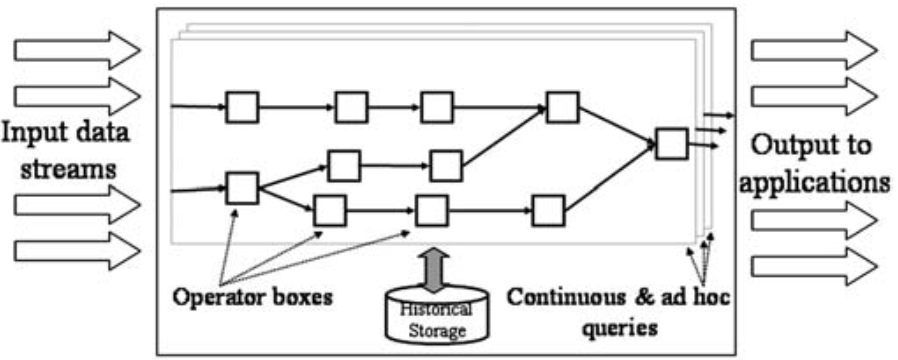
\includegraphics[width=3.5in]{./img/AuroraSystemModel.png}
\caption{Aurora's system model~\cite{Aurora2003}.}
\label{fig_aurora_system}
\end{figure}

The Aurora system was designed following the assumptions for DSMS. As seen in Fig.~\ref{fig_aurora_system}, the system model follows a boxes-and-arrows approach. After data from multiple sources have arrived at the system, different operators modify the data to generate one or more outputs. The operators are connected to each other by the user, thus providing the ability to form complex queries. One operator may have multiple outputs. Additionally, a historical storage might be used for persisting interesting information or for setting recovery points. Historical storage is organized as a B-tree. Users can set up and manage the system with a graphical user interface. Input data sources can be computer programs or sensors. The data arrive in form of tuples, with one field of each tuple serving as a unique identifier.

To satisfy different needs to access the data stream, Aurora provides three different types of queries. The user is (1) able to define continuous queries. Furthermore, the system (2) supports views that might include historical data. Finally, users can perform (3) ad-hoc queries to receive information not included in the continuous queries.

\begin{figure}[!t]
\centering
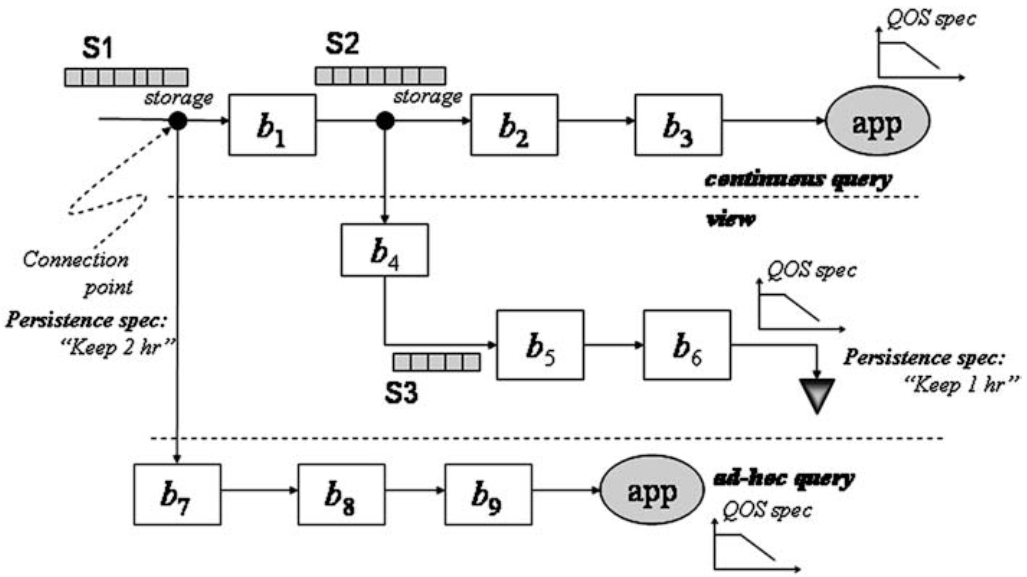
\includegraphics[width=3.5in]{./img/AuroraQueryModel.png}
\caption{Aurora's query model~\cite{Aurora2003}.}
\label{fig_aurora_query_model}
\end{figure}

Fig. ~\ref{fig_aurora_query_model} shows Aurora's query model. Each box represents an operator, the connecting arrows represent the data flow. There are predefined connection points, represented by the dots, i.e. before \textit{b\textsubscript{1}}, and between \textit{b\textsubscript{1}} and \textit{b\textsubscript{2}}. Each connection point possesses a dedicated storage (\textit{S1, S2}), and ad-hoc queries might be connected only to a connection point. For every connection point's dedicated storage the time of persistence can be configured individually. This storage enables ad-hoc queries and views on historical data. One operator may have multiple outputs. In such a case, a subnetwork is created for each output. Further subnetworks are created, when new queries are connected to connection points. Also note that each operator has its own output buffer, which can be accessed by the succeeding operators.

\subsection{Optimization in Aurora}\label{auroraOptimization}
Optimizers of RDBMSs aim to minimize the number of iterations over large data sets. When handling streams, a system needs to process data as it arrives. The amount of computation per arriving tuple is small, but the optimizer expects a high number of operations. Also, the data arrival rates might be enormous. Aurora's optimizer focuses on two areas. 

The first area is the optimization of continuous queries. The system gathers runtime statistics, such as cost of box execution and box selectivity, i.e. the relative number of output tuples per input tuple. Three optimization tactics are employed. First, Aurora aims to reduce the size of each tuple, by using projections as early as possible. This way, the system eliminates unused operators. Second, combining operators might improve execution speed by getting rid of box-execution overhead. Map and filter operations may be combined with almost all other operators (more on the different operators in Section~\ref{squal}). Last, if two operators commute, they can be safely reordered. The optimizer reorders two operators, if the resulting amount of computation is smaller than before reordering. We define two boxes \textit{b\textsubscript{i}} and its successor \textit{b\textsubscript{j}}. Each operator's execution cost is \textit{c(b\textsubscript{i})} and \textit{c(b\textsubscript{j})} and their selectivities \textit{s(b\textsubscript{i})} and \textit{s(b\textsubscript{j})}. The optimizer reorders the operators, if \eqref{eq_aurora_optimizer} is fulfilled:

\begin{equation}
c(b\textsubscript{i})+c(b\textsubscript{j})*s(b\textsubscript{i})>c(b\textsubscript{j})+c(b\textsubscript{i})*s(b\textsubscript{j})\label{eq_aurora_optimizer}
\end{equation}

To make use of the aforementioned optimization tactics, the optimizers periodically performs the following algorithm.

\begin{enumerate}\label{enum_optimization_algorithm}
\item Select subnetwork to optimize.
\item Find all connection points surrounding the subnetwork.
\item Hold all input messages at connection point before the subnetwork (upstream).
\item Drain all messages out of the subnetwork through connection points following the subnetwork (=ownstream).
\item Optimize by moving selections, combining boxes and reordering operators. This creates a new subnetwork.
\item Connect new network to the connection points and route the data through the network. 
\item Repeat periodically.
\end{enumerate}
This algorithm makes sure that no tuples are lost and that the system can resume its operation seamlessly.

When the user schedules an ad-hoc query, the second area of the optimizer is utilized. If the query accesses historical data, the optimizer is able to perform indexed lookups on the B-tree of the historical storage. This works for filter and join operations and only, if the B-tree is indexed on the fields corresponding to the user's query.

\subsection{Runtime Operation in Aurora}\label{auroraRuntime}

\begin{figure}[!t]
\centering
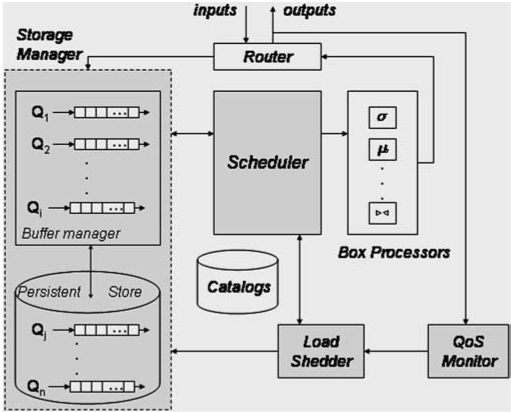
\includegraphics[width=3.5in]{./img/AuroraRuntime.png}
\caption{Overview on Aurora's runtime components~\cite{Aurora2003}.}
\label{fig_aurora_runtime}
\end{figure}

Fig. ~\ref{fig_aurora_runtime} shows the different components Aurora employs at runtime. We will focus on the Quality of Service Monitor, Storage Manager and Scheduler.

\begin{figure}[!t]
\centering
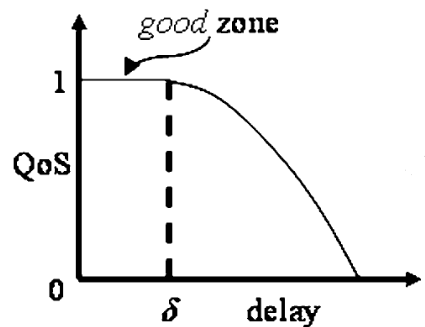
\includegraphics[width=1.5in]{./img/AuroraQoS.png}
\caption{Quality of Service in relation to the input-output delay~\cite{Aurora2003}.}
\label{fig_aurora_qos}
\end{figure}

For evaluating the performance of the system, Aurora employs a Quality of Service (QoS) Monitor. The user may define multiple functions, which specify the decline of the QoS in relation to different, user defined, metrics. At least one function, i.e. showing the decline of QoS in relation to the time delay between a tuple arriving and being put out of the system, must be implemented. Fig. ~\ref{fig_aurora_qos} shows the mandatory function. Extending this, other functions, such as the percentage of delivered tuples ore more complex metrics, such as QoS for each value of the output, meaning a change of the abscissa metric, might be added. The QoS Monitor continuously gathers runtime statistics to evaluate the QoS by using the user defined functions as performance indicators.

Because disk I/O operations are expensive, the Aurora Storage Manager's (ASM) task is to minimize the amount disk I/O. The ASM works in two areas. First, it performs queue management. As stated above, each operator has a queue at its output, which is shared by all directly succeeding operators. Each succeeding box maintains two pointers on its preceding queue. One is the head, which marks the oldest tuple in the queue not yet processed by the operator. The other is the tail, which marks the oldest tuple that is not needed by the operator anymore. Head and tail define the window of tuples that an individual operator needs from the queue. Older values might be discarded. The queues are organized in 128kB blocks and may be increased or decreased block-wise in times of overflow or underflow. The ASM has a buffer pool in main memory, where it can load blocks of queues.

To keep track of which queue-blocks to keep in main memory the developers created a tabular data structure that is shared by the Scheduler and ASM. Each row represents one operator box and has different attributes, i.e. scheduling priority (maintained by the Scheduler), percentage of its queue currently in main memory (maintained by ASM) and a flag indicating if the box is running. When the ASM discovers a block of a queue in main memory that is not currently running, it loads a block of a queue with higher priority instead. Also, when main memory space is needed for a block from disk, the block belonging to the lowest priority queue gets replaced. This ASM-workflow results in top prioritized boxes most often being already in main memory when needed.

Another task of the ASM is connection point management. To be more efficient, ASM performs insertions and deletions to the historical storage in batches.

\begin{figure}[!t]
\centering
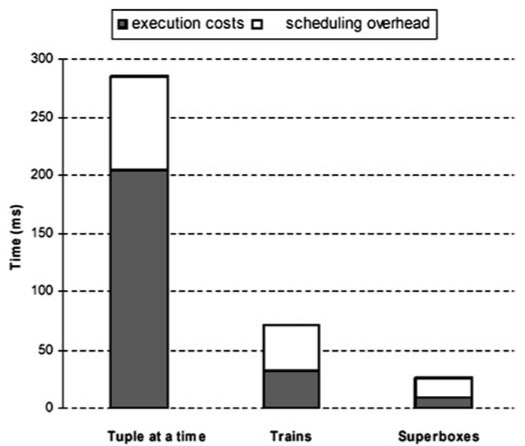
\includegraphics[width=2.5in]{./img/AuroraSchedulingPerformance.png}
\caption{Influence of scheduling tactics on end-to-end tuple processing time~\cite{Aurora2003}.}
\label{fig_aurora_scheduling_performance}
\end{figure}

In addition to storage management, the scheduling of operations is of importance. There are several issues that the Scheduler must address to achieve good overall performance.  The potentially large scale of the system and real-time requirements describe the frame, in which the Scheduler operates. Also, there might be dependencies between box executions that the Scheduler needs to keep track of. Finally, the system can not schedule solely on QoS specifications, because that might lead to exploding end-to-end tuple processing costs. The number of box calls per tuple as well as I/O operations should be minimized. To meet these requirements, the Scheduler uses two tactics. First, it generates \textit{tuple trains}, which means that it queues as many tuples as possible before processing them and processes each train as a whole. Second, the trains are processed by as many consecutive boxes as possible at once. This tactic is called \textit{superbox scheduling}. Both tactics work exceptionally well and increase end-to-end processing time drastically. Execution costs as weill as scheduling overhead are reduced, as shown in Fig.~\ref{fig_aurora_scheduling_performance}.

If there is a system overload, the Load Shedder is able to use QoS information and employ two tactics to increase performance. It is able to drop tuples and also filter tuples. The problem with dropping tuples is that there are more important and less important tuples (which may or may not be specified by a user created QoS function). This issue is addressed by the tactic of filtering tuples, which tries to use QoS information to drop less important tuples.

\subsection{Stream Query Algebra}\label{squal}
To define queries for Aurora's operator boxes, the developers have created a new declarative query language, called Stream Query Algebra (SQuAl). It consists of eight explicit operators, which are similar to other established query languages. The reason for creating a new query language has been that data streams have some characteristics, because of which traditional data manipulation languages are not applicable. For example, aggregating operators work different, when they are executed on possibly infinite streams. SQuAl operators are classified into order agnostic and order sensitive ones.

There are three order agnostic operators in SQuAl: \textit{map}, \textit{filter} and \textit{union}. \textit{Map} serves as a generalized projection and is able to manipulate each attribute of an incoming tuple. Hence, it is able to change the schema of a processed tuple. \textit{Filter}, on the other hand, does not change the schema of a tuple, but applies user defined predicates to different attributes. It is able to route tuples to different output streams based on a predicate, which means that filter can serve as a fan-out operator. On the other hand, \textit{union} combines two or more streams with a common schema into one stream, therefore serving as a fan-in operator. The tuples themselves are not changed by \textit{union}.

The order sensitive operators are \textit{Bsort},\textit{ aggregate}, \textit{join} and \textit{resample}. Because of their nature – performing operations on a set of tuples – it is important to specify an \textit{order} and a window in which tuples must arrive. To satisfy this need, the user must specify an order function \textit{O}(On \textit{A}, Slack \textit{n}, GroupBy \textit{B\textsubscript{1}}, …, \textit{B\textsubscript{i}}) for each operation in addition to the basic function of the operation itself. \textit{A} is the attribute in which the order is assumed, \textit{n} defines a possible slack (default is \textit{n = 0}) and \textit{B\textsubscript{a,…,i}} are attributes on which the input is grouped by. With a nonzero slack, the restriction on the assumed arrival order can be relaxed. With a slack of \textit{n = 2}, a window of \textit{size 3} is defined for the respective operator. Considering the \textit{Bsort} operator, which orders input tuples of a stream, the slack defines the buffer size for ordering tuples. With a \textit{slack of 2}, the buffer has three fields on which \textit{Bsort} performs the ordering. This means that out of order tuples, which arrive up to two tuples late, can be put into order. With \textit{aggregate}, a user defined aggregation of several values is possible. To take into account that there is an infinite stream of tuples \textit{aggregate} needs a specified window, after which it performs the aggregation. It also needs a step function, which defines how the window advances. The \textit{Join} operator joins tuples of two streams together on a user defined predicate \textit{P} and a defined window \textit{size} for an attribute. For example, the user could join two streams of position data of two cars, that were in the same area (\textit{P}) within a given time (\textit{Size}). The \textit{resample} operator performs an interpolation for each value on a stream \textit{S\textsubscript{1}} based on values in a stream \textit{S\textsubscript{2}}. As \textit{join} and \textit{aggregate}, \textit{resample} also needs a window, on which it operates. Last, there is an implicit \textit{split} operation that is performed by simply connecting a box not to one, but to several other boxes, thus splitting the output into several disjunct streams.

\subsection{Areas for Improvement in Aurora}\label{auroraImprovement}
Aurora presented a new approach to handling data streams. Many ideas were new, and the performance of the system was excellent compared to RDBMSs. But nevertheless, the developers identified two fields for further improvement. First, Aurora does neither support parallel, nor distributed execution. It lacks the ability to dynamically scale out in times of heavy load. Another problem with running only on one system is that the whole system shuts down when the computer has a problem. This issue was addressed in further research. \textit{Medusa} was developed as a distributed execution engine for aurora. Both projects were combined to form \textit{Borealis}~\cite{AuroraBorealis2016}, a distributed stream processing engine. The project was commercialized in 2003 as StreamBase Inc.

Another inconvenience is that Aurora's operator set is not extensible. In an enterprise environment, being able to add operators for specific business needs might be of interest.

Furthermore, the developers aimed to address the ability of Aurora ``to cope with missing and imprecise data values, which are common in applications involving sensor-generated data streams"~\cite{Aurora2003} in further research.